\subsection{Analytic 2x2}


\subsubsection{Microstates 2x2}

\begin{center}
\label{tab:states-2x2}
\captionof{table}{This shows the different microstates that is possible for a 2x2 spinmatrix. It also states the energy and magnetic moment for each microstate.}
\begin{tabularx}{\textwidth}{c c c X c c c}
    \hline 
    \hline 
        State & Energy & Magnetic moment && State & Energy & Magnetic moment \\ 
    \hline
        \tilstand{1}{1}{1}{1} & -8J & 4 && \tilstand{0}{0}{0}{0} & -8J & -4 \\ \\
        
        \tilstand{0}{1}{1}{1} & 0J & 2 && \tilstand{1}{0}{0}{0} & 0J & -2 \\ \\
        \tilstand{1}{0}{1}{1} & 0J & 2 && \tilstand{0}{1}{0}{0} & 0J & -2 \\ \\
        \tilstand{1}{1}{0}{1} & 0J & 2 && \tilstand{0}{0}{1}{0} & 0J & -2 \\ \\
        \tilstand{1}{1}{1}{0} & 0J & 2 && \tilstand{0}{0}{0}{1} & 0J & -2 \\ \\

        \tilstand{0}{0}{1}{1} & 0J & 0 && \tilstand{1}{1}{0}{0} & 0J & 0 \\ \\ 
        \tilstand{0}{1}{0}{1} & 0J & 0 && \tilstand{1}{0}{1}{0} & 0J & 0 \\ \\
        \tilstand{1}{0}{0}{1} & 8J & 0 && \tilstand{0}{1}{1}{0} & 8J & 0 \\ \\
    \hline
\end{tabularx}
\end{center}



\begin{center}
\label{tab:states-2x2-summary}
\captionof{table}{The table shows a summary from table \ref{tab:states-2x2}. }
\begin{tabularx}{\textwidth}{c X c X c X c}
    \hline 
    \hline 
        Number of $\color{red}{\uparrow}$ && Multiplicity && Energy && Magnetic moment \\ 
    \hline
        4   &&      1      &&      -8J     &&       4       \\  
        3   &&      4      &&      0J      &&       2       \\
        2   &&      2      &&      8J      &&       0       \\
        2   &&      4      &&      0J      &&       0       \\
        1   &&      4      &&      0J      &&       -2      \\
        0   &&      1      &&      -8J     &&       -4      \\
    \hline
\end{tabularx}
\end{center}












\pagebreak
\subsubsection{Quantities}

We will use the equations from section \ref{sec:expect}.
\\
\\
For energy the eq. \ref{eq:E} will result in:

\begin{align*}
    &Z = \sum_i = e^{-\beta E_i}
    \\
    &\text{T = kT/J = 1} 
    \\
    &Z = \sum_i = e^{-\beta E_i} = 2e^{8} + 2e^{-8} + 12
\end{align*}


For energy the eq. \ref{eq:E} will give the result:

\begin{align*}
    &\langle E \rangle = \sum_i E_iP(E_i)
    \\
    &\text{T = kT/J = 1} 
    \\
    &\langle E \rangle = \frac{1}{Z} \sum_i E_i e^{-E_i}
    \\
    &\langle E \rangle = \frac{1}{Z} \left( 16 e^8 - 16e^{-8} \right) = 7.9839
    \\ 
    &\langle E \rangle /N= \frac{\langle E \rangle}{4} = 1.9959
\end{align*}


For energy the eq. \ref{eq:M} will give the result:

\begin{align*}
    &\langle |M| \rangle = \sum_i M_iP(E_i)
    \\
    &\text{T = kT/J = 1} 
    \\
    &\langle |M| \rangle = \frac{1}{Z} \sum_i M_i e^{-E_i}
    \\
    &\langle |M| \rangle 
    = 
    \frac{1}{Z} 
    \left(
      4\cdot1e^{8} 
    + 2\cdot4e^{0} 
    + 0\cdot2e^{-8} 
    + 0\cdot4e^{0} 
    + 2\cdot4e^{0}  
    + 4\cdot1e^{8}
    \right) 
    \\
    &\langle |M| \rangle 
    = 
    \frac{1}{Z} 
    \left(
    16
    + 8 e^{8}
    \right) = 3.9946
    \\ 
    &\langle |M| \rangle /N= \frac{\langle M \rangle}{4} = 0.9986
\end{align*}

For $C_V$ we need to calculate $\langle E^2 \rangle$:

\begin{align*}
    &\langle E^2 \rangle = \sum_i E_iP(E_i)
    \\
    &\text{T = kT/J = 1} 
    \\
    &\langle E^2 \rangle = \frac{1}{Z} \sum_i E_i^2 e^{-E_i}
    \\
    &\langle E^2 \rangle = \frac{1}{Z} \left( 128 e^8 + 128 e^{-8} \right)
    \\
    &C_V = \langle E^2 \rangle - \langle E \rangle^2 = 0.12832
    \\ 
    &C_V/N = 0.03208
\end{align*}



For $\chi$ we need to calculate $\langle M^2 \rangle$:

\begin{align*}
    &\langle M^2 \rangle = \sum_i M_i^2P(E_i)
    \\
    &\text{T = kT/J = 1} 
    \\
    &\langle M^2 \rangle = \frac{1}{Z} \sum_i M_i^2 e^{-E_i}
    \\
    &\langle M^2 \rangle 
    = 
    \frac{1}{Z} 
    \left(
      16\cdot1e^{8} 
    + 4\cdot4e^{0} 
    + 0\cdot2e^{-8} 
    + 0\cdot4e^{0} 
    + 4\cdot4e^{0}  
    + 16\cdot1e^{8}
    \right) 
    \\
    &\langle M^2 \rangle 
    = 
    \frac{1}{Z} 
    \left(
    32
    + 32 e^{8}
    \right) = 15.9732
    \\
    &\text{$\langle M \rangle$ is 0 which makes $\langle \chi \rangle = \langle M^2 \rangle$}
    \\
    &\langle \chi \rangle = 15.9732
    \\
    &\langle \chi \rangle / N = 3.9933
\end{align*}

Below you can see a summary for the quantities:

\begin{align*}
    \langle E \rangle /N &= 1.9959  \qquad &&\langle |M| \rangle /N = 0.9986
    \\
    C_V/N &= 0.03208  \qquad &&\langle \chi \rangle / N = 0.004010
\end{align*}









\pagebreak
\subsection{example}

\begin{figure}[H]
    \centering
    \begin{subfigure}{0.5\textwidth}
        \centering
        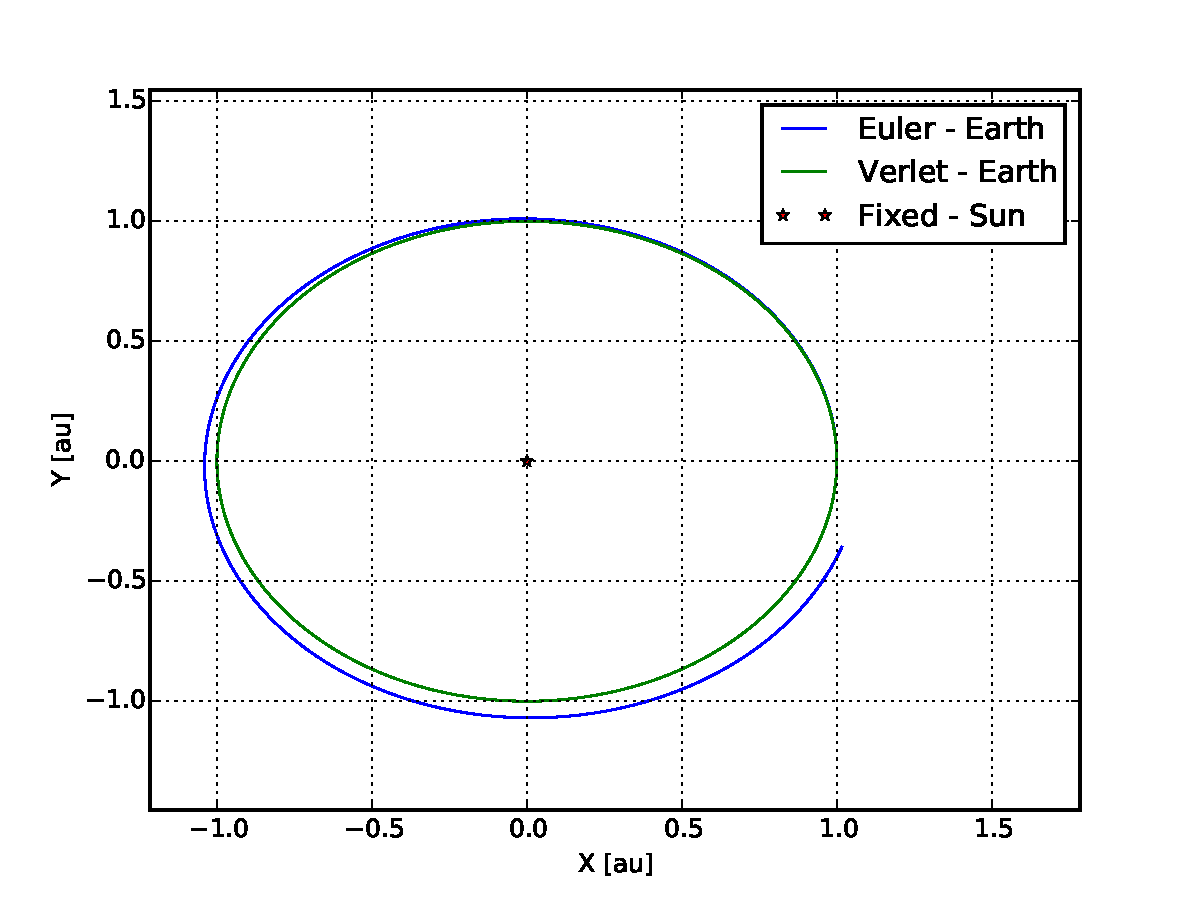
\includegraphics[width=\linewidth]{result/bilder/earth-sun.pdf}
    	\caption{}
    \end{subfigure}%
    ~ 
    \begin{subfigure}{0.5\textwidth}
        \centering
        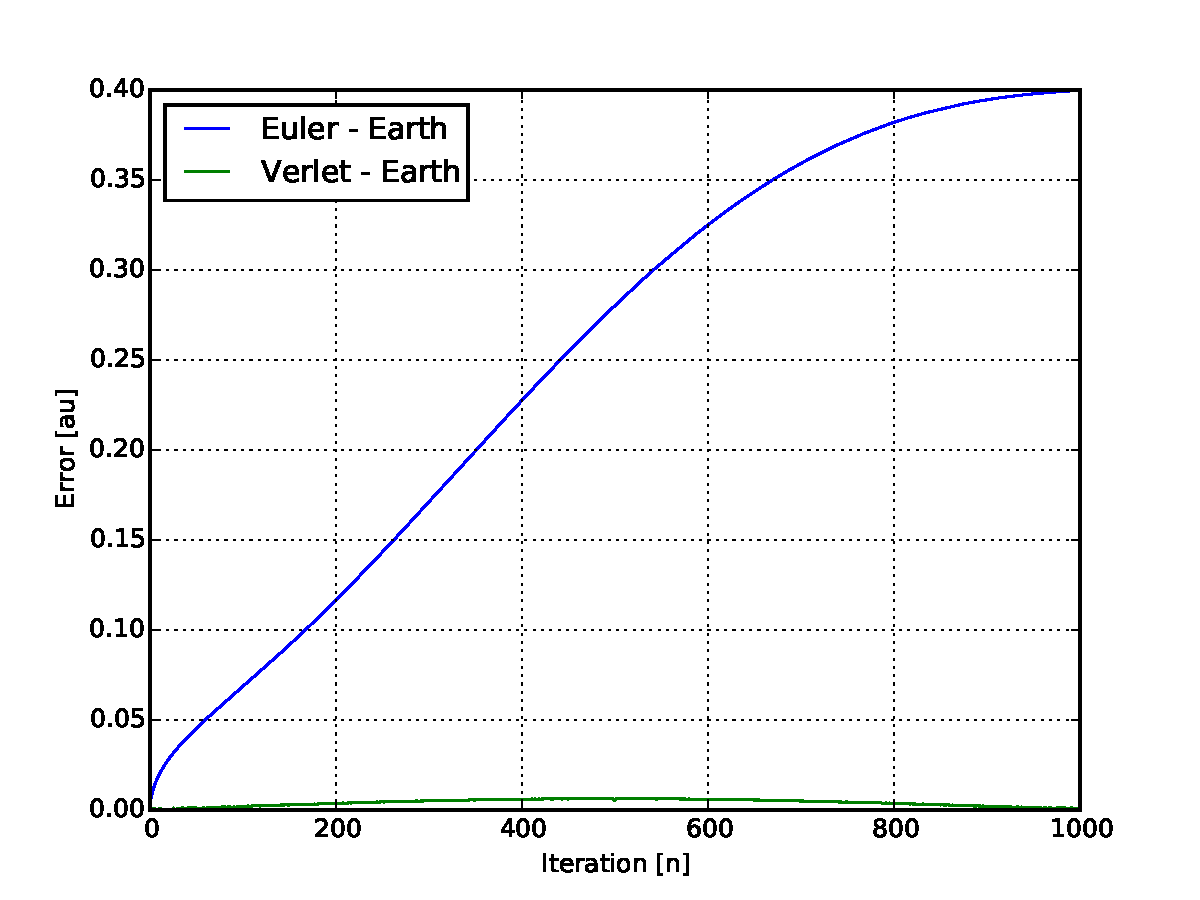
\includegraphics[width=\linewidth]{result/bilder/earth-sun-error.pdf}
        \caption{}
    \end{subfigure}
    \caption{a) shows the orbit of earth around the sun. The intial velocity is set to $2\pi$ in y direction and the start position to 1 au in x direction. b) shows how the error develops. The intial values should give a perfect circular motion. So the error is calculated by $r_i - r_{0}$. It is apparent that the Verlet-Velocity method is a better approximation. This simulation was with 1000 points with the end time of 1 year. Both simulations was produced by \href{https://github.com/erikfsk/Project-3/tree/master/Project3/earth-sun-standard-results}{\textcolor{blue}{plot\_earth\_sun.py}}}
    \label{fig:earth-sun}
\end{figure}
